\documentclass[a4paper,12pt,french]{article}

\usepackage[cours]{../../Style}

%\selectcolormodel{cmyk}

%\usepackage{wrapfig}

% Début du document
%%%%%%%%%%%%%%%%%%%
\begin{document}

\title{Dérivation}
\maketitle

\begin{programme}
\item Point de vue local:
\begin{itemize}
\item Sécantes à une courbe passant par un point donné, taux de variation en un point
\item Tangente à une courbe en un point, définie comme position limite des sécantes
\item Nombre dérivé en un point défini comme limite du taux de variation
\item Equation réduite de la tangente en un point.
\end{itemize}
\item Point de vue global
\begin{itemize}
\item Fonction dérivée
\item Dérivées de $x \mapsto x^2$, $x \mapsto x^3$, de combinaisons linéaires, de polynômes de degré $\leq 3$
\item Sens de variation d'une fonction, lien avec le signe de la dérivée
\item Tableau de variations, extremums
\end{itemize}
\item Capacités
\begin{itemize}
\item Interprétation du nombre dérivé comme coeff directeur de la tangente
\item Construire la tangente à une courbe en un point
\item Déterminer l'équation réduite de la tangente à une courbe en un point
\item Calculer la dérivée d'un polynome de degré $\leq 3$
\item Déterminer le sens de variation et les extremums d'une fonction polynome de degré $\leq 3$
\end{itemize}
\end{programme}

\rem{Manque l'équation de la tangente (bof?).\\
Première partie sur les sécantes, le programme a l'air d'être clair sur ce point... (sera distribué, résumé sur un fichier géogebra et fait rapidement)\\
Variations que à la fin, dommage?\\
Vocabulaire: tangente à la courbe de $f$ passant par $A$ un peu lourd}

\section{Nombre dérivé}

\subsection{Sécantes et tangentes}

%Tangente, lim des sécantes. Lecture graphique de la dérivée
\begin{defin}
\compo[0.5]
{
Soit $f$ une fonction, avec $A$ et $M$ deux points sur la courbe de $f$ d'abscisses respectives $a$ et $a+h$.

La droite $(AM)$ est une \textbf{sécante} de la courbe de $f$.

Son coefficient directeur vaut: $$\frac{\text{déplacement vertical}}{\text{déplacement horizontal}}=\frac{f(a+h)-f(a)}{h}$$

Ce nombre correspond au taux d'accroissement de $f$ entre $a$ et $a+h$.
}
{
\begin{center}
\begin{tikzpicture}
\begin{axis}[
styleglobal,
width=0.9*\linewidth,
xmin=-3, xmax=4,
ymin=-1, ymax=4,
xtick distance=1,
ytick distance=1,
ticks=none,
declare function={f(\x)=e^(0.75*(\x-1)-0.5);}
]
\addplot[styleplot]{f(x)} node [pos=0.8,left] {$\mathscr C_f$};
\node[stylepoint,fill=blue,label=above:$A$] (A) at (0.5,{f(0.5)}) {};
\node[stylepoint,fill=blue,label=above left:$M$] (B) at (3,{f(3)}) {};
%
\draw[color=blue,dashed,very thick] (0.5, 0) -- (A) node [pos=0,below] {$a$};% -- (0,{f(0.5)}) node [pos=1,left] {$f(x)$};
\draw[color=blue,dashed,very thick] (3, 0) -- (B) node [pos=0,below] {$a+h$};% -- (0,{f(1.2)}) node [pos=1,left] {$f(y)$};
\draw[<->,color=DarkGreen,densely dashed,ultra thick] (0.5,0) -- (3,0) node[pos=0.5,below] {$h$};
%
\draw[color=blue,dashed,very thick] (0,{f(0.5)}) -- (A) node [pos=0,left] {$f(a)$};% -- (0,{f(0.5)}) node [pos=1,left] {$f(x)$};
\draw[color=blue,dashed,very thick] (0,{f(3)}) -- (B) node [pos=0,left] {$f(a+h)$};% -- (0,{f(1.2)}) node [pos=1,left] {$f(y)$};
\draw[<->,color=DarkGreen,densely dashed,ultra thick] (0,{f(0.5)}) -- (0,{f(3)}) node[pos=0.5,left] {$f(a+h)-f(a)$};
%
\draw[line width=1.3pt,shorten <= -20cm,shorten >= -20cm,densely dotted] (A) -- (B);
\end{axis}
\end{tikzpicture}
\end{center}
}
\end{defin}

\begin{propr}
\compo
{
A mesure que $M$ se rapproche du point $A$ (autrement dit lorsque $h$ se rapproche de $0$), la droite $(AM)$ se rapproche d'une autre droite, appelée \textbf{tangente de $\mathscr C_f$ en $A$}, qui épouse la courbe de $f$ près de $A$. De plus, le nombre $\frac{\text{déplacement vertical}}{\text{déplacement horizontal}}=\frac{f(a+h)-f(a)}{h}$ se rapproche du coefficient directeur de cette tangente.
}
{
\begin{center}
\begin{tikzpicture}
\begin{axis}[
styleglobal,
width=0.9*\linewidth,
xmin=-3, xmax=4,
ymin=-1, ymax=4,
xtick distance=1,
ytick distance=1,
ticks=none,
declare function={f(\x)=e^(0.75*(\x-1)-0.5);}
]
\addplot[styleplot]{f(x)} node [pos=0.75,below right] {$\mathscr C_f$};
\node[stylepoint,fill=blue] (A) at (0.5,{f(0.5)}) {};
\node[stylepoint,fill=blue,inner sep=1.3pt] (B) at (2.5,{f(2.5)}) {};
\node[stylepoint,fill=blue,inner sep=1.5pt] (C) at (1.5,{f(1.5)}) {};
\node[stylepoint,fill=blue,inner sep=1.7pt] (D) at (0.75,{f(0.75)}) {};
\node[stylepoint,fill=blue,inner sep=1.9pt] (E) at (0.625,{f(0.625)}) {};
\draw[color=blue,dashed,thick] (0.5, 0) -- (A) node [pos=0,below] {$a$};% -- (0,{f(0.5)}) node [pos=1,left] {$f(x)$};
\draw[color=blue,dashed,thick] (2.5, 0) -- (B) node [pos=0,below] {$a+h$};% -- (0,{f(1.2)}) node [pos=1,left] {$f(y)$};
\draw[color=blue,dashed,thick] (1.5, 0) -- (C);
\draw[color=blue,dashed,thick] (0.75, 0) -- (D);
\draw[color=blue,dashed,thick] (0.625, 0) -- (E);
\draw[thick,shorten <= -20cm,shorten >= -20cm,densely dotted] (A) -- (B);
\draw[thick,shorten <= -20cm,shorten >= -20cm,densely dotted] (A) -- (C);
\draw[thick,shorten <= -20cm,shorten >= -20cm,densely dotted] (A) -- (D);
\draw[line width=1.3pt,shorten <= -20cm,shorten >= -20cm,densely dotted] (A) -- (E);
\addplot[styleplot,color=Crimson,ultra thick]{0.75*e^(0.75*(-0.5)-0.5)*(x-0.5)+f(0.5)};
\end{axis}
\end{tikzpicture}
\end{center}
}
\end{propr}

\begin{ex}
\compo[0.7]
{
On se donne la fonction $f:x \mapsto x^2$, et le point $A(1;1)$ sur $\mathscr C_f$. Soit $h \in \R$. On a $f(1)=1$ et $f(1+h)=(1+h)^2=1+2h+h^2$. Alors:

$$\begin{aligned}\frac{f(1+h)-f(1)}{h}&=\frac{1+2h+h^2-1}{h}\\
									 &=\frac{2h+h^2}{h}\\
									 &=2+h \end{aligned}$$
Cette quantité se rapproche de $2$ lorsque $h$ tend vers $0$. Alors le coefficient directeur de la tangente à la courbe de $f$ passant par $A$ est $2$.
}
{
\begin{tikzpicture}
\begin{axis}[
styleglobal,
width=0.9*\linewidth,
xmin=-1, xmax=3,
ymin=-1, ymax=3,
xtick distance=1,
ytick distance=1,
minor x tick num=0,
minor y tick num=0,
declare function={f(\x)=\x^2;}
]
\addplot[styleplot] {f(x)} node[pos=0.76,left] {$\mathscr C_f$};
\node[stylepoint,fill=blue,label=above right:$A$] (A) at (1,{f(1)}) {};

\addplot[styleplot,densely dashed,color=DarkBlue] {{2*(x-1)+f(1)}};
\end{axis}
\end{tikzpicture}
}
\end{ex}

\rem{Voir fichier géogebra}

\subsection{Lecture du nombre dérivé}

\begin{defin}
On appelle nombre dérivé de $f$ en $a$, noté $f'(a)$, le coefficient directeur de la tangente à la courbe de $f$ au point d'abscisse $a$.
\end{defin}

\begin{ex}
\compo[0.5]
{\setlength{\parskip}{1ex}
On a représenté une fonction $f$ ci-contre.

Pour obtenir $f'(2)$, on place $A$ défini comme le point de $\mathscr C_f$ d'abscisse $2$, puis on détermine le coefficient directeur de la tangente de $\mathscr C_f$ passant par $A$. On a alors $f'(2)=-1$.

Pour obtenir $f'(-1)$, on place $B$, et on détermine le coefficient directeur de la tangente associée: $f'(-1)=2$. En utilisant l'ordonnée à l'origine, on en déduit que l'équation de cette tangente est $y=2x+3$.
}
{
\begin{center}
\begin{tikzpicture}
\begin{axis}[
styleglobal,
width=0.9*\linewidth,
xmin=-3, xmax=5,
ymin=-1, ymax=4,
xtick distance=1,
ytick distance=1,
minor x tick num=1,
minor y tick num=1,
declare function={f(\x)=-0.5*(\x-1)*(\x-1)+3;}%0.2*\x*(\x+2)*(\x-3);}
]
\addplot[styleplot] {f(x)} node[pos=0.76,left] {$\mathscr C_f$};
\node[stylepoint,fill=blue,label=above right:$A$] (A) at (2,{f(2)}) {};
\node[stylepoint,fill=blue,label=above left:$B$] (B) at (-1,{f(-1)}) {};

\draw[color=blue,dashed,very thick] (2, 0) -- (A);%node [pos=0,below] {$a$};
\draw[color=blue,dashed,very thick] (-1, 0) -- (B);% node [pos=0,below] {$a+h$};

\addplot[styleplot,densely dashed,color=DarkBlue] {{-1*(x-2)+f(2)}};
\addplot[styleplot,densely dashed,color=DarkRed] {{2*(x+1)+f(-1)}};

\draw[->,thick,color=DarkBlue] (A) -- (4,{f(2)});
\draw[->,thick,color=DarkBlue] (4,{f(2)}) -- (4,0.5);
\draw[->,thick,color=DarkRed] (B) -- (-1,3);
\draw[->,thick,color=DarkRed] (-1,3) -- (0,3);

\end{axis}
\end{tikzpicture}
\end{center}
}
\end{ex}

%Formule générale avec schéma

\section{Fonction dérivée}

\subsection{Généralités, règles de calcul}

\begin{defin}
On définit la fonction dérivée de $f$, notée $f'$, qui à $x$ associe le coefficient directeur de la tangente à la courbe de $f$ au point d'abscisse $x$.
\end{defin}

\begin{prop}
On a les dérivées usuelles suivantes:
\begin{center}\renewcommand{\arraystretch}{1.5}
\begin{tabularx}{5cm}{|Y|Y|} \hline
$f(x)$ & $f'(x)$ \\ \hline
$k \in \R$ & $0$ \\ \hline
$x$ & $1$ \\ \hline
$x^2$ & $2x$ \\ \hline
$x^3$ & $3x^2$ \\ \hline
\end{tabularx}
\end{center}
\end{prop}


\begin{prop}
Soient $f$ et $g$ deux fonctions, et $\lambda \in \R$. Alors:
\begin{itemize}
\item $(f+g)'=f'+g'$
\item $(\lambda f)'=\lambda f'$
\end{itemize}
\end{prop}

\begin{ex}
Soit $f:x \mapsto {\color{DarkRed}x^2}+{\color{DarkBlue}2x}+{\color{black}1}$. Alors $f'(x)={\color{DarkRed}2x}+{\color{DarkBlue}2 \times 1} + {\color{black}0} =2x+2$.
\end{ex}

%$f(x)=\tikzmark{cube} \ 2x^{\tikzmark{expcube} 3}-\tikzmark{carre}3x^{\tikzmark{expcarre} 2}+5\cancel{x} \cancel{-1}$

%\tikz[remember picture]{\draw[overlay,->] (pic cs:expcube) to[bend right=80] (pic cs:cube);}
%\tikz[remember picture]{\draw[overlay,->] (pic cs:expcarre) to[bend right=10] (pic cs:carre);}

\subsection{Lien avec les variations}

\begin{thm}
Soit $f$ une fonction et $a \in \R$, $b \in \R$.
\begin{itemize}
\item Si $f'$ est positive sur $[a;b]$, alors $f$ est croissante sur $[a;b]$.
\item Si $f'$ est négative sur $[a;b]$, alors $f$ est décroissante sur $[a;b]$.
\item Si $f'$ est nulle sur $[a;b]$, alors $f$ est constante sur $[a;b]$. Les zéros de $f'$ correspondent aux extremums de $f$. (A reformuler)
\end{itemize}
\end{thm}

\begin{app}
On peut alors dresser le tableau de variations d'une fonction grâce au tableau de signes de sa dérivée.
\end{app}

\begin{ex}
\compo[0.52]
{\setlength{\parskip}{1ex}
Soit $f:x \mapsto x^2-4x+2$. Alors $f'(x)=2x-4$.

On a $f'(x)=0$ ssi $2x=4$ ssi $x=2$. (On peut aussi calculer $\frac{-b}{a}$).

On a de plus $f(2)=2^2-4 \times 2+2=4-8+2=-2$.

Cela donne alors:
}
{
\begin{centrer}
\begin{tikzpicture}
\tkzTabInit[lgt=1.5,espcl=2.2]{$x$ /1, $f'(x)$/1, $f(x)$/2}{$- \infty$, $2$, $+ \infty$}
\tkzTabLine{,-,z,+}
\tkzTabVar{+/$ $, -/$-2$, +/$ $}
\end{tikzpicture}
\end{centrer}
}
\end{ex}
\end{document}
